\documentclass[10pt,twoside,a4paper]{article}
\usepackage[IL2]{fontenc} % lepšia sadzba písmena Ľ než v T1
\usepackage[utf8]{inputenc}
\usepackage{graphicx}
\usepackage{url} % príkaz \url na formátovanie URL
\usepackage{hyperref} % odkazy v texte budú aktívne (pri niektorých triedach dokumentov spôsobuje posun textu)

\usepackage{cite}

\pagestyle{headings}
\title{Procedural Game Content Generation Using the Wave Function Collapse Algorithm\thanks{Semester project in the subject Methods of engineering work, if. year 2022/23, management: Name Surname}}
\author{Martin Dinja\\[2pt]
	{\small Slovak University of Technology in Bratislava}\\
	{\small Faculty of Informatics and Information Technologies}\\
	{\small \texttt{xdinja@stuba.sk}}
}

\date{\small 30. september 2022}

\begin{document}

\maketitle

\tableofcontents

\begin{abstract}
    \begin{center}
        This thesis deals with the generation of game content using the Wave Function Collapse algorithm. 
    \end{center}
\end{abstract}

\section{Introduction}\label{sec:introduction}

% An Introduction to the application of the wave function collapse algorithm for procedural generation of game content.
Procedural content generation (PCG) is a general term for a system that follows some patterns and generates an output based on those patterns.
Its use case is generating assets or content that would be too time-consuming to create manually.
PCG is mainly connotatively tied to game content generation, but its use cases can be more creative.
Most PCG systems use game-specific assets with game-specific rules and algorithms to generate their content.
A more general application fit for a wide range of games is the Wave Function Collapse algorithm developed by Maxim Gumin \cite{WFC}.
Wave Function Collapse is a greedy PCG algorithm based on the concept of collapsing a wave function, which is a mathematical representation of a quantum state.
This method can generate a large, high-quality, consistent output from a small set of input patterns.
It can be used in various applications, although its most commonly used for generating 2D tilemaps for games.
It can also generate 3D models, music, poetry, and more.
WFC's output can only be as good as its input, so it's essential to have a good set of input patterns and rules. 
My goal in this thesis is to create a simple, configurable application that will use the WFC algorithm to generate tilemaps for games, given a user-defined set of input patterns and rules.


\section{Theory}\label{sec:theory}
As mentioned in the introduction [\ref*{sec:introduction}], the Wave Function Collapse algorithm is a greedy PCG algorithm based on the concept of collapsing a wave function, which is a mathematical representation of a quantum state.
A function starts in a superposition of values and collapses when that function is measured.
The result of the measurement is the value of the function at that point.
So applying that to the PCG of a 2D tilemap, first, we need to define a set of input patterns and their rules concerning each other.
Then the algorithm will assign each tile a superposition of all possible patterns.
After prepending the superpositions, the algorithm will assign one random pattern to a tile with the least superpositions, also known as the least entropy, effectively collapsing its wave function, which is also why it is called a collapse algorithm.
Then we reevaluate all the affected tiles and their possible patterns and remove the ones that don't fit the rules.
Then we repeat the process until there is no more entropy in the tilemap.

\section{Implementation}\label{sec:implementation}
% subsections: Preparation, infrastructure, algorithm, GUI.
\subsection{Preparation}\label{sec:preparation}
% The preparation of the project.
JavaScript was chosen as the language to implement the WFC algorithm primarily for its workflow and comfort.
And for the GUI, I chose p5js, a JavaScript library for creating graphics and animations.
It has a simple and easy-to-use API, and it's fast enough for this project.

After deciding on the language and the library, I started by creating tile images and developing a rule system for them.
The rule system, rather than detailing every relation to every possible rotation of every tile, uses an array of four numbers representing a connection type for each side of the tile. \texttt{[top, right, bottom, left]}.
Only the same connection types are allowed to connect to each other.

With that, we can start implementing the infrastructure for the algorithm.

\subsection{Infrastructure}\label{sec:infrastructure}
% The infrastructure of the project.
The infrastructure of the project is the core of the algorithm.
It makes it easier for the central part of the algorithm to work with the tilemap.
It also contains the main functions of the algorithm.

The infrastructure consists of many functions aiding the algorithm.
The most important ones are the ones that work with the tilemap.

The configuration with the rules and the tile images is stored in JSON, detailing each tile's name, picture path, and allowed connections.

Foremost, we need to parse all the patterns and their rules into a format with which the algorithm can interface.
We do this by going through each pattern, rotating it, and writing each rotation into a hash map in the form \texttt{ct1\_ct2\_ct3\_ct4: [name, img, connections:[], rotate]}. 
With that, we get a hash map of all the possible rotations of all the patterns.

From the hash map, we create a two-dimensional array of objects which contain the tile's superposition, entropy, and collapse state.
The superposition is an integer array of all assignable patterns, the entropy is the number of superpositions, and the collapse state is a boolean value that tells us if the tile is collapsed or not.

Then we only have smaller helper functions for getting a tile's entropy, getting the least entropy tile, collapsing a tile, reevaluating a tile's rules, examining the validity between two tiles, and checking if the tilemap has entirely collapsed.

When updating a cell with the \texttt{updateCell} function, we first grab all of the neighboring tiles and their superpositions.
Then we go through each neighbor, filtering out the states that fit with none of the neighbors' states.
And finally, if the cell remains with only one pattern, we collapse it.

Rule checking is especially vital to the algorithm, even though it's very straightforward.
In the \texttt{isRuleFollowed} method we take in three parameters, state A, state B, and the direction in which A connects to B.
If the connection type of A in the direction is the same as the connection type of B in the opposite direction, then the rule has been followed.
In addition to more specific rules, we check if B's tile can be connected to A's tile.
To ensure that even if the connection types are the same, tile A still needs to allow connection to tile B, preventing non-compatible tiles from connecting. For instance, if you don't want to prohibit the same tile from connecting to itself.

Other GUI-oriented functions are described in the GUI section [\ref*{sec:gui}].

Now let's go over the central part of the algorithm.


\subsection{Algorithm}\label{sec:algorithm}
% The main part of the project.
The central part of the project is the algorithm itself.
It uses the helper, interface, and infrastructure functions to work with the tilemap.
We start by parsing the JSON file into a hash map and preloading all the needed tile images.
Then we create the tilemap and fill each tile's state array with all possible states.
Then we start the main loop of the algorithm.
In the loop, we get the tile with the least entropy, collapse it, and reevaluate all the affected cells.
Evaluating the cells is done by updating the states of each neighbor of the collapsed cell, then reevaluating the states of their neighbors, and so on, until we reach a point where cell states don't change any more.
Finally, we check if all of the cells are collapsed, and if they are, the algorithm halts.
Otherwise, we repeat the loop.

\subsection{GUI}\label{sec:gui}
% The GUI of the project.
The GUI of the project is a simple interface for the user to view the satisfying progression of the algorithm.
Its core is a p5js instance that draws the tilemap.
Here we only have two functions. 
The most important one is the \texttt{drawGrid} function, which draws the grid.
Second is the \texttt{drawImg} function, which draws an image given the coordinates, size, and angle.

There are also different options for how and what the GUI will draw.
We can disable the constant drawing and instead draw it only when the algorithm has finished.
We can also opt-in to draw every possible cell state of a non-collapsed cell.

\subsection{Modifications}\label{sec:modifications}
% Modifications to the algorithm.
The algorithm is very simple and straightforward, but it can be modified to fit different needs.
For a more controlled distribution of tile types we can assign a weight value to each type.
The weight value will be used to determine the likelihood of a tile being collapsed into a certain pattern.

We can also expand WFC with generic search, giving it the ability to generate levels targeting specific play experiences.
This is the topic of a paper released by Raphael Bailly and Guillaume Levieux\cite{BL22}.

There is also a way to augment the algorithm with the Growing Grid neural network for procedural map generation \cite{NMBP20}

We can take control to another level and introduce more constraints to the algorithm making the output seem more Human-Designed.
As detailed in the paper by Darui Cheng, Honglei Han, and Guangzheng Fei\cite{CHF20}.

\section{Results}\label{sec:results}
% subsections: examples, performance, conclusions.
With the algorithm implemented, we can now generate tilemaps.
Starting off with a simple example (Figure~\ref{fig:example1}).
\begin{figure}[h]
    \centering
    
\includegraphics[width=0.5\textwidth]{figures/road_tiles.png}
    \caption{Example 1}\label{fig:example1}
\end{figure}

Defining the rules for these tiles, we can generate a 10 by 10 tilemap with the following result (Figure~\ref{fig:example1map}):

\begin{figure}[h]
    \centering
    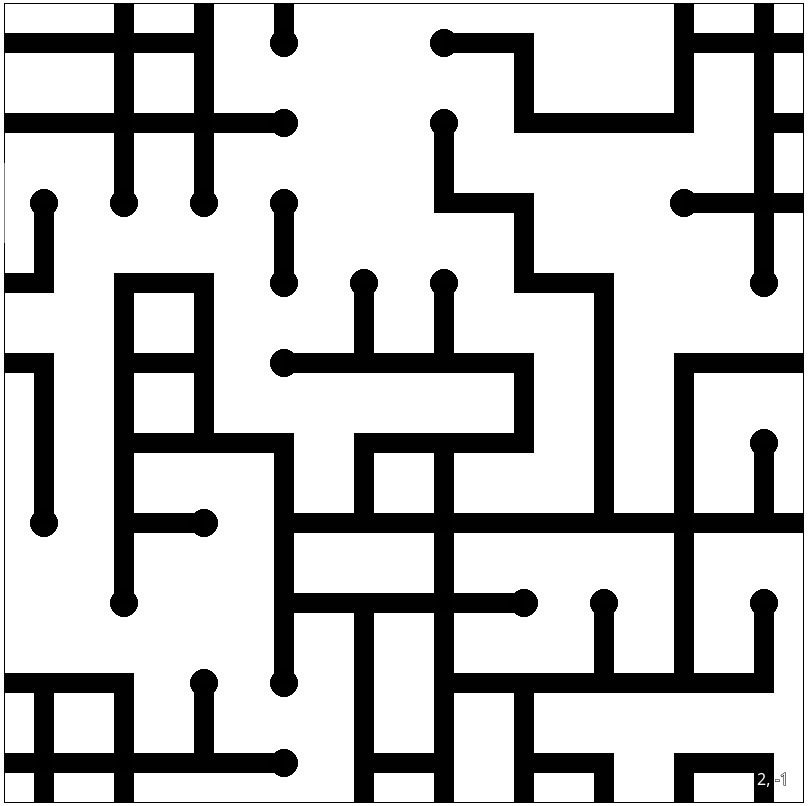
\includegraphics[width=0.5\textwidth]{figures/roads_output.png}
    \caption{Example 1 map}\label{fig:example1map}
\end{figure}


\section{Comparison with other methods}\label{sec:comparison}
\section{Conclusion}\label{sec:conclusion}
% \cite{BL22}
% \cite{CHF20}
% \cite{KLL+19}
% \cite{LRGC22}
% \cite{NMBP20}
\bibliography{lit}
\bibliographystyle{alpha}

\end{document}
